\documentclass[../main-00.tex]{subfiles}
\begin{document}

\chapter{Data and Processing Volume Estimates \hideme{Schellman, Junk, Muether}}
\label{ch:est}
\fixme{Heidi: moved tables of numbers from intro to here.  Still needs better organization}
In this chapter we will describe the assumptions that go into a bottoms-up estimate of data volumes and describe possible methods of reducing the total volumes while retaining physics capabilities. 

\section{Introduction}

% \begin{dunetable}
% [Data Sizes and Rates]
%  {l |r r r }
%  {tab:volumes}
%  {Data sizes and rates for different processes in each far detector module.  Uncompressed data sizes are given. As readouts will be self-triggering an extended 5.4 ms readout window is used instead of the 3ms for the triggered \dword{pdsp} runs.  We assume beam uptime of 50\% and 100\% uptime for non-beam science. These numbers are derived from references \protect{\cite{bib:docdb16028}}and \protect{\cite{bib:docdb14983}}.}
% % 5
%  Process & Rate/module & \qquad size/instance &\qquad  size/module/year\\ \toprowrule
%  %
%  Beam event & 41/day & 6 GB&47 TB/year\\
%  Cosmic rays &4,500/day&  6 GB& 9.7 PB/year\\
%  Supernova trigger& 1/month& 115 TB& 1.4 PB/year\\
%  Calibrations&2/year&750 TB& 1.5 PB/year\\
%  %\toprowrule 
%  Total& & &12.9 PB/year\\
%  \end{dunetable}




%  \subsection{Supernova candidates}


%  \begin{figure}
%  \begin{center}
%  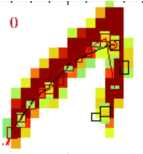
\includegraphics[height=0.3\textwidth]{graphics/IntroFigures/Fig_10a_Picture3.png} \hskip 1 in
% 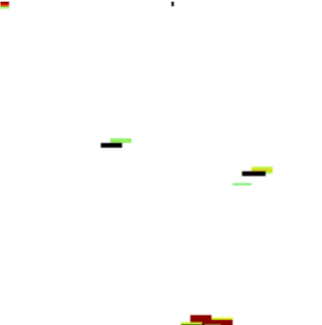
\includegraphics[height=0.5\textwidth]{graphics/IntroFigures/Fig_10b_Picture4.png}
%  \caption{Left) a charged current interaction of a 30 MeV energy electron neutrino in the DUNE Far Detector.  Right) a neutral current excitation and de-excitation of an Ar nucleus by a  10 MeV neutrino.}
%  \label{blips}
%  \end{center}
%  \end{figure}


% Supernova candidates pose a unique problem for data acquisition and reconstruction.  Supernova physics in DUNE is discussed in some detail in the \dword{tdr}\cite{ Abi:2020evt} and only summarized here. A classic core-collapse supernova 10 kpc away would be expected to yield around 3,000  charged-current electron neutrino interactions across 4 detector modules.  The oscillation physics is not fully understand and can result in significant modulations of the event rates for different neutrino types  over the few tens of seconds of the burst.  DUNE's fine-grained tracking should allow significant pointing power with the most optimistic scenario of four modules and high electron neutrino fraction yielding pointing resolutions of less than 5 degrees.   Figure \ref{blips} illustrates simulated signatures of supernova neutrino interactions in the far detector. The ability to produce a reasonably fast pointing signal would be extremely valuable to optical astronomers doing followup, especially if a supernova was in a region where dust masks the primary optical signal.   The need to be alert to supernovae and to quickly transfer and process the data imposes significant requirements on triggering, data transfer and reconstruction beyond those imposed by the more regular beam-based oscillation physics.   For example, a compressed supernova readout of all four modules will be of order 184 TB in size and take a minimum of 4 hrs to transfer over a 100 Gbs network,  and then take of order 130,000 CPU-hrs for signal processing at present speeds.  If processing takes the same time as transfer, a peak of 30,000 cores would be needed. 


% \fixme{Move or copy to the data volumes section}
% \begin{dunetable}
% [Useful FD Data Quantities]
% {|l  l |c       | l |}
% {tab:exec-comp-bigpicture-es}
% {Useful quantities for computing estimates for \dword{sp}
% readout. For  sparse \dword{fd} events, the pattern recognition phase, which scales with occupancy is expected to be substantially faster than the signal processing phase which scales with detector size.  }%
% Quantity&&\qquad Value \qquad&Explanation\qquad \qquad\\
% \toprowrule
% {\bf Far Detector Beam:}&&&\\ 
% &Single APA readout &41.5 MB& Uncompressed 5.4 ms\\ 
% &Single APA readout &16.6 MB& $\times 2.5$ compression\\
% &APAs per module& 150&\\
% &Full module readout &6.22  GB& Uncompressed 5.4 ms\\ 
% &Beam rep. rate&0.83 Hz&Untriggered\\  
% Signal processing &CPU time/APA&40 sec&from MC/ProtoDUNE\\  
% Signal processing &CPU time/input MB& 2.5 sec/MB& compressed input\\
% &Memory footprint/APA&0.5-1 GB&ProtoDUNE experience\\  
% \toprowrule
% {\bf Supernova:}&&&\\
% &Single channel readout &300 MB& Uncompressed 100 s\\  
% &Four module readout& 460 TB& Uncompressed 100 s\\  
% &Trigger rate&1  per month&(assumption)\\
% \end{dunetable}


% \dword{dune} requires a global software and computing effort to store, catalog, reconstruct, calibrate and analyze approximately 30 PB of data/year from  multiple \dword{lartpc} detectors containing 17 kT of liquid each,  a larger scale than any previous neutrino experiment. Single event sizes are expected to range from 200 MB for the existing \dword{protodune} experiments running at \dword{cern}, to 6 GB for a far detector module, to 460 TB for a full readout of a 100 s supernova candidate across 4 modules. Full sensitivity to neutrino oscillations, supernovae neutrinos,  and beyond the standard model phenomena  require precise energy calibration and energy thresholds in the few MeV range, which present significant challenges for signal processing.  In addition to the general distributed computing issues that are common to large \dword{hep} experiments, the very large event sizes present  \dword{dune} with a unique computing challenge.  \dword{dune} intends to benefit from previous experience and will contribute to ongoing improvements in general \dword{hep} computing infrastructure, working in collaboration with the \dword{osg}, the \dword{wlcg} , and the \dword{hep} Software Foundation among others.  However, the unique nature of    \dword{dune} events will require dedicated effort to adapt and integrate   \dword{dune}-specific solutions to achieve the physics goals of the experiment.

%\subsection{Near Detectors}
% \subsection{Near Detectors}

% High precision oscillation physics requires a near detector system to allow measurement of the original neutrino flux and improved understanding of neutrino interaction physics.  The DUNE  collaboration is proposing a suite of near detectors optimized for these two goals. 
 
%  The near detectors will be located in an enclosure on the Fermilab site 574 meters from the target and will be exposed to the DUNE neutrino beam.    Interaction rates per spill (at 0.83 Hz) are expected to be very large, with 40-60 interactions per spill, including muons originating from interactions in material upstream of the fiducial volumes. Figure \ref{beamline} shows the beamline and location of the near detectors on the Fermilab site. There are three major subsystems:
%  A pixel readout liquid argon detector, \dword{ndlar}, is  the most upstream of the three sub-detectors shown in Figure \ref{nd}, where the beam propagates  from right to left. Immediately downstream of \dword{ndlar} is the gaseous liquid argon detector, \dword{ndgar}, which serves \dword{ndlar} as  a muon spectrometer and allows more detailed study of neutrino interactions that occur within its gas volume. Beyond \dword{ndgar}, is the \dword{sand} component of the ND that acts as a beam monitor. %Figure \ref{nd} shows the three \dword{nd} subdetectors in the near enclosure. 
 
%  \begin{figure}[ht]
%      \centering
%      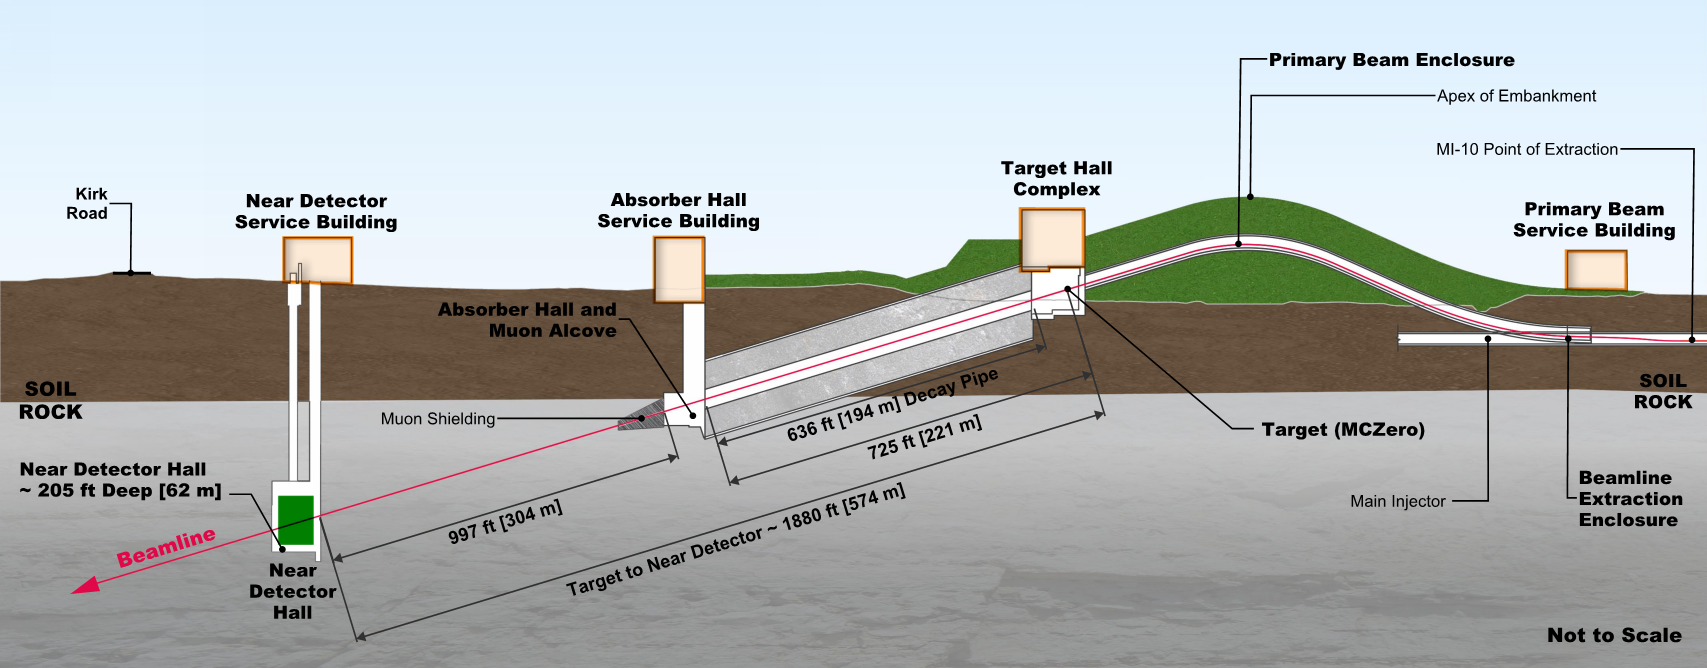
\includegraphics[height=0.3\textwidth]{graphics/IntroFigures/beamline-sideview.png}
%      \caption{The LBNF neutrino beamline on the Fermilab site. The near detectors will be situated 574 m from the target and 62 m below grade.}
%      \label{beamline}
%  \end{figure}
 
%  \begin{figure}[ht]
%      \centering
%      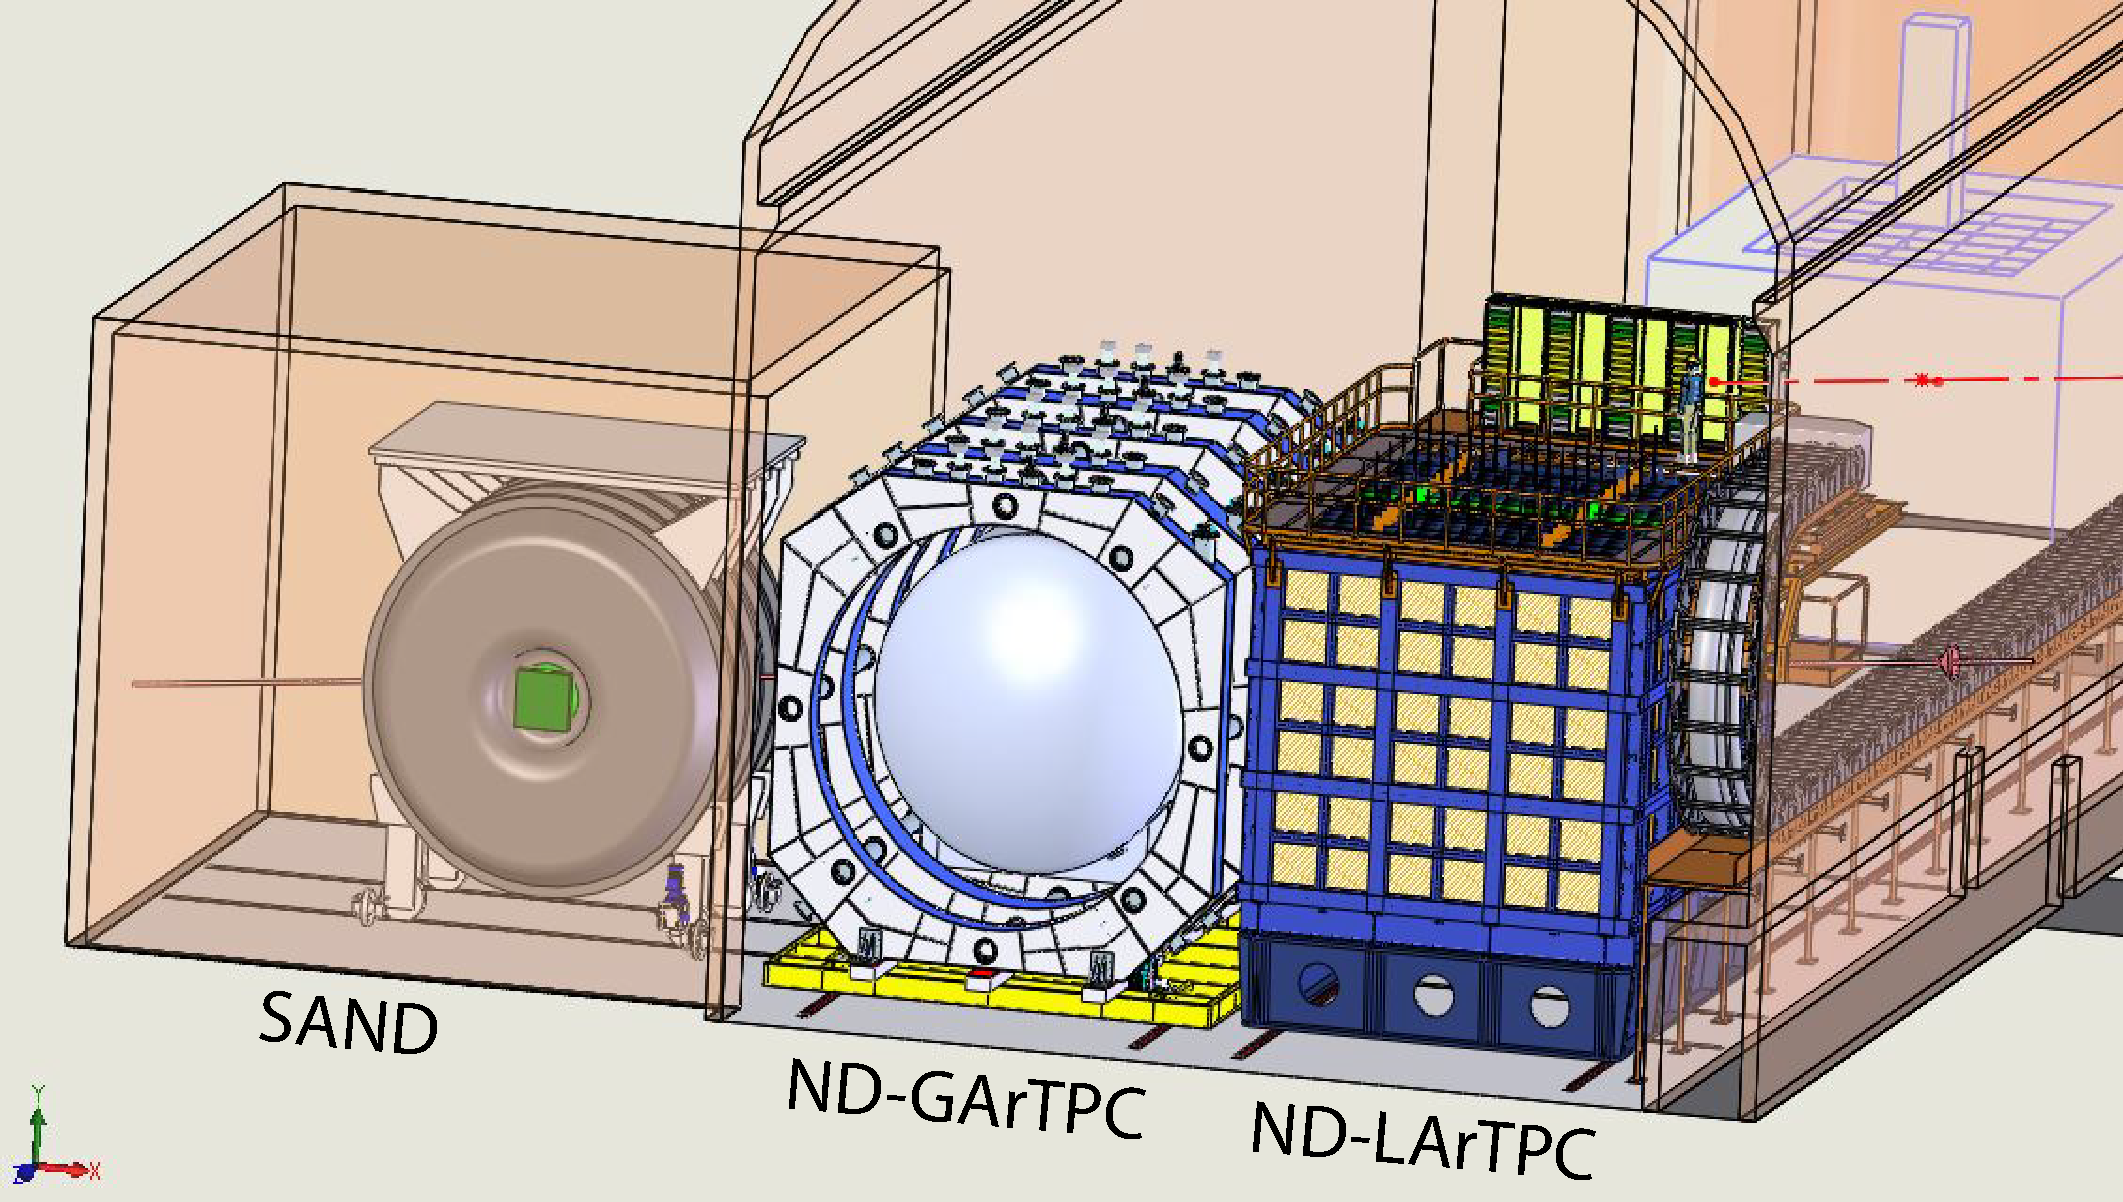
\includegraphics[height=0.5\textwidth]{graphics/IntroFigures/All3Detectors.pdf}
%      \caption{The near detector systems in an on-axis configuration.  The beam enters from the lower right in this view. The \dword{sand} scintillating beam monitor remains at beam center while the pixel ND-LAr TPC detector and gaseous ND-GAr TPC detectors can be moved off-axis to make detailed studies of the neutrino flux at multiple angles.  }
%      \label{nd}
%  \end{figure}
 
%  \subsubsection{pixel LArTPC - ND-Lar}
 
%  As the target material in the Deep Underground Neutrino Experiment (DUNE) far detectors is liquid argon, optimal cancellation of systematic uncertainties between the near and far detectors requires that the near detector include a liquid argon component to match the \dword{fd}.  However, at the intense neutrino flux and high event rate in the ND region, occupancies will be too high to allow the 2-D readout provided by conventional wire planes. A new ArgonCube  technology has been developed that allows pixelized charge readout  and provides unambiguous 3D imaging of  particle interactions.  The ND-LAr component of the DUNE ND is made up of a configuration of ArgonCube LArTPCs  large enough to provide the required hadronic shower containment and statistics.  %The 5 m (along beam)×7 m (horizontal,  transverse to beam)×3 m (height), 67 t fiducial mass, of ND-LAr are optimized primarily for  hadronic containment under the assumption that ND-GAr will measure the sign and momentum  of downstream exiting muons. Figure 2.2 shows the arrangement of modules in the crystat for  ND-LAr.  Section 2.2 gives a discussion of the physics consideration
 
%  The pixel liquid argon detector will have 12~million $3\times 3$~mm$^2$ pixel channels and $\sim$4200~photon detector channels.  The LArTPC will read out only pulse times and integrals, in contrast to the far detector which reads out every time slice.  The photon detectors will, however, read out complete wave-forms.   A total of 3~MB of uncompressed data is anticipated per spill from the TPC with 5-MB from the photon detectors leading to an estimate of 144 TB/year for uncompressed in-spill data. Calibrations and cosmic ray data increase that data volume by around 20\%.

% % For calibrations, 300 runs are assumed to be taken per year, each generating 10~GB of data, for the TPC, and a similar set of runs for the photon detectors.  These runs include pulser runs, laser runs, radioactive source runs, or other special-condition runs that require taking data outside of the regular spills.  Since they are not tied to the spill timing structure, they can be collected at higher trigger rates and take less time.

% % In addition to the beam data, cosmic rays will contribute to the data volume.  For the \dword{ndlar} geometry in the ND hall, the anticipated rate
% % of cosmic rays is 100~Hz.  If all cosmic ray data were collected, the data volume would be approximately 1~MB/sec.  The scenario considered here is to
% % collect one spill's worth of cosmic ray data for every ten beam spills, for a data volume of 6.3 TB per year.  While the activity on the cosmic-ray triggers is expected to be much less than that on a beam spill, it is assumed that the cosmic-ray triggering will continue even when the beam is off.

% % The TPC-only out-of-spill and calibration numbers have been scaled by 8/3 to account for photon detector data, assuming full waveform readout in these samples, yielding the same ratio as in-spill data and the same compression. 

% \subsubsection{Near Detector Gaseous Argon TPC}
% \label{sec:comp-dataestimates-mpd}

% The \dword{ndgar} is a magnetized detector system consisting of a high-pressure gaseous argon TPC  (HPgTPC) surrounded by an electromagnetic calorimeter (ECAL) and a muon system. The \dword{ndgar} measures the momentum and sign of charged particles exiting the ND-LAr. In addition, for neutrino interactions occurring in the \dword{ndgar} itself, higher resolution and lower momentum thresholds can be achieved for charged particle tracks, leading to improved neutrino interaction models. This capability enables further constraints of systematic uncertainties for long-baseline neutrino  oscillation analyses.

% The \dword{ndgar} is composed of 678,136 readout pads in the TPC, and approximately 3~million channels in the \dword{ecal}.  Approximately one in five spills will generate an interaction in the gas TPC, but particles entering the gas from interactions in the \dword{ecal} will provide the bulk of the data volume.  The readout strategy will be similar to the LArTPC, with only time and integral recorded. A  data volume of 2 MB of uncompressed data per spill is expected from the TPC.  The calorimeter is expected to contribute approximately 1~MB per spill of uncompressed data.

% % For calibrations, 300 runs per year generating 10~GB of data per run are assumed for the TPC, and a similarly-sized set of calibration runs are assumed for the \dword{ecal}.  Cosmic rays are expected to be collected between spills and when the beam is off.



% \subsubsection{SAND}
% \label{sec:comp-dataestimates-sand}
% %The 3rd detector subsystem is the \dword{sand}, a scintillator based monitor, consists of a 3-D pixelated scintillator detector, an electromagnetic calorimeter and XXX

% The \dword{sand} component of the near detector (ND)'s primary function is the primary beam flux monitor.   SAND consists of an active scintillator target \dword{3dst} followed by a tracking system immersed in a solenoidal superconducting magnet  and  a $4\pi$ electromagnetic calorimeter.

% \dword{sand}'s \dword{3dst} calorimeter component is composed of 11,520,000 $1\times 1\times 1$~cm$^3$ scintillating cubes, read out by 153,600 fibers.  There are expected to be approximately 2,160 hits per spill with a total of 0.13 MB of data per spill.  The  \dword{ecal}~\cite{Adinolfi:2002zx} uses 4,850 PMTs, with an estimated 5,500 total hits per spill or 33 kB of packed data per spill.   The data volume from SAND is 4.3 TB/year with these assumptions.  The amount of data from out-of-spill cosmic rays is estimated to be 20\% of that of the in-spill data, or approximately 1 TB.  The data volume from SAND is significantly smaller than that from the \dword{ndlar} and the \dword{ndgar} due to the relative sizes of the three-dimensional tracking volumes and the segmentation choices.

%\fixme{Move this to the Data volumes section}
%\subsubsection{CPU needs and simulation}

% Table \ref{tab:nd_data_volume_estimates} summarizes the expected data sizes from the near detector. Due to the much higher data density in the near detector, CPU times/beam spill are expected to be much higher and are estimated to be 300 CPU/sec/spill using current processors for $1.5\times 10^7$ spills/year. Simulated data samples will need to be an order of magnitude larger and thus require at least 10 times the CPU power.  This leads to a rough estimate of CPU needed of approximately 3,000 core-years/year.

% \begin{dunetable}[Near Detector Data Estimates]
% {l r}
% {tab:nd_data_volume_estimates}
% {Annual DUNE near detector data volume estimates.  No compression is assumed.}
% Type & Volume/year\\ \toprowrule
%     {\bf \dword{ndlar}}     &  \\
%     \quad\quad In-spill data & 144 TB \\
%     \quad\quad Out-of-spill cosmics & 16 TB\\
%     \quad\quad Calibration & 16 TB\\
%     \quad\quad Total & 176 TB \\\toprowrule
%     {\bf \dword{ndgar}}           & \\
%     \quad\quad In-spill data & 52 TB \\
%     \quad\quad Out-of-spill cosmics & 10 TB \\
%     \quad\quad Calibration & 6 TB\\
%     \quad\quad Total & 68 TB \\\toprowrule
%     {\bf \dword{sand}}        & \\
%         \quad\quad In-spill data & 4 TB\\
%     \quad\quad Out-of-spill cosmics & 1 TB\\
%     \quad\quad Calibration & 1 TB \\
%     \quad\quad Total & 6 TB \\\toprowrule
%     {\bf Total ND} & {\bf 250 TB}\\
% \end{dunetable}

% \begin{dunetable}
% [CPU estimates for Near Detector]
% {l r}
% {tab:NDCPUPerEvent}
% {Preliminary CPU estimates per event for the DUNE near detector components, in seconds.}
% Type&time/event\\ \toprowrule
%     {\bf LArTPC} &  \\
%     \quad\quad Monte Carlo gen+sim & 100 s \\
%     \quad\quad Reconstruction & 60 s\\\toprowrule
%   {\bf MPD} &  \\
%     \quad\quad Monte Carlo gen+sim & 100 s\\
%     \quad\quad Reconstruction & 12 s\\\toprowrule
%     {\bf SAND} & \\
%     \quad\quad Monte Carlo gen+sim & 100 s\\
%     \quad\quad Reconstruction & 10 s\\\toprowrule
% \end{dunetable}

% A Conceptual Design Report for the Near Detector systems is in preparation and the \dword{nd} computing efforts are being integrated with the existing far detector and protoDUNE efforts. 

%{\it borrowed from TDR to test bib/glossary/units}


% \section{Comments and Conclusions}
% This discussion has centered on the acquisition and fast processing of raw data from novel and extremely large liquid argon time projection chambers. Many other computing challenges lie ahead but were beyond the scope of this paper.  These include

% \begin{description}
% \item[{\bf Simulation:}] particle propagation in liquid argon is reasonably fast to simulate as there are not complicated volume boundaries to cross but simulating electron drift trajectories (and scintillation light trajectories) in a diffusive, electron absorbing, moving medium immersed in a non-uniform  electric field remains a challenging computational challenge. 
% \item[{\bf Near detectors:}] a suite of near detectors are needed to characterize the neutrino beam as it originates at Fermilab.  These detectors are still being developed but will introduce a large number of differing detector technologies.  While individual interactions are likely to be much smaller than readouts of the far detectors, the beam cycle is of order 1 Hz and each readout will contain multiple cosmic ray and beam interactions.
% \item[{\bf Data analysis:} ] The small (order 100) group of \dword{pdsp} and \dword{pddp} and \dword{dune} developers and analyzers have successfully analyzed the beam and cosmic ray data and performed simulations needed to produce the physics sections of the \dword{tdr}.  We expect analysis of the full experiment to involve many more individuals and much more data.  A campaign of training for new users and design of a suite of efficient analysis tools is needed.  We have initial prototypes based on NOvA and MicroBooNE analysis. 
% \end{description}

% Fortunately, \dword{dune} is able to take advantage of the huge and heroic developments in software and computing made for the Intensity Frontier and LHC experiments over the past decade.  We have demonstrated that, even with preliminary versions of our tools and algorithms, we can quickly reconstruct and analyze data from large liquid argon TPC's at full rate. We look forward to an exciting and fruitful next decade. 



% Test using \dword{tms}
%%%%%%%%%%%%%%%%%%%%%%%%%%%%%%%%
\section{Assumptions}
\label{sec:est:assume}  %% fix label according to section

\subsection{Raw data assumptions}
DUNE's detectors will produce information from a variety of technologies.  We anticipate that raw data volumes will be dominated by the digitized waveforms from liquid argon detectors and, to a lesser extent, photon detectors, in \dword{pd}, the \dword{fd} and the \dword{nd}.  
These raw data volumes can be reduced by the \dword{daq} system by several means.


\begin{itemize} 
\item triggered readout of particular time slices
\item triggered readout of particular geographic regions
\item lossless zero suppression
\item lossy zero suppression
\item hardware pattern recognition
\end{itemize}

Overall, we assume that the above methods can reduce data volumes from the hundreds of Exabytes that would be produced by continuous readout to a manageable 30 PB/year. 

\subsection{Derived data assumptions}


 \begin{dunetable}[Data Retention Policies]{llrrrr}{tab:est:retention}
{Retention policies by data tier}
Tier&Description&Tape copies& Lifetime &Disk Copies& Lifetime\\
Raw & Physics data& 2 & indefinitely & 1 & 1 year\\
Test & test and commissioning & 1 &6 months &1 & 6 months \\
Hits & reconstructed hits & 1 & 10 years & 1 & 1 month \\
Reco & pattern recognition &1 & 10 years & 2 & 2 years\\
\end{dunetable}

\section{ProtoDUNE}
\label{sec:est:ProtoDUNE}  

Our estimates  are largely based on our experience with the single and double-phase \dword{pd} detectors which ran at CERN in late 2018.  The \dword{pdsp} detector used \dword{hd} \dword{tpc} technology read out 6 \dwords{apa} and a mix of photon detectors while the first far detector module will have 150 \dwords{apa} and photon detectors based on the \dword{arapuca} technology.  Data rates and assumptions for protoDUNE have been documented in \href{docdb:20515}{https://docs.dunescience.org/cgi-bin/private/ShowDocument?docid=20515}.  Table \ref{tab:est:usefulpd} provides useful quantities for data volumes derived from the ProtoDUNE experience. 

 \begin{dunetable}[Useful quantities for computing far detector data volumes]{lrr}{tab:est:usefulpd}
{Useful quantities for computing estimates for \dword{sp}
readout.   }%\rowtitlestyle
Quantity&Value&Explanation\\
\toprowrule
%{\bf Far Detector Beam:}\\ \colhline
Number of channels/APA&2,560&\\
Readout time & 3 ms&\\
\# of time slices & 6000&\\
Single APA readout &23 MB& Uncompressed  estimate\\ \colhline
APAs & 6 &\\
Full detector readout &178 MB& Uncompressed real \\ \colhline
Full detector readout &71 MB& Compressed real \\ \colhline
Effective compression factor &2.5&\\ \colhline
Beam rep. rate&4.5 Hz&Average\\ \colhline
Hit reconstruction time CPU time/APA& 30 sec&from MC/ProtoDUNE\\ \colhline
Pattern recognition time CPU time event & 400 sec&from MC/ProtoDUNE\\ \colhline
Simulation time CPU time event & 2700 sec&from MC/ProtoDUNE\\ \colhline
Memory footprint/APA&0.5-1GB&ProtoDUNE experience\\ \colhline
\end{dunetable}

 

For example, uncompressed single phase data from ProtoDUNE-SP were observed to be around 178 MB in size, which is the amount expected for the number  of TPC channels read + a 20\% overhead for other detectors and headers.  Compressed SP data averages 71 MB, consistent with compression by a factor of 2.5.  

Dual phase data includes 2 CRPs for the 2019 run.  Observed data size without compression  was 110MB.  %Numbers for 2018 and 2019 have been 

For the far detector with APA's we assume 






[DUNE-doc-20515-v9]

\section{FD}
\label{sec:est:FD}  

For \dword{hd} far detector data volumes, we use our \dword{pdsp} experience and assume that raw data sizes and hit finding CPU times scale with the number of \dwords{apa} while pattern recognition and simulation times scale with the number of interactions. 

 \begin{dunetable}[Useful quantities for computing \dshort{hd} data volume
estimates]{lrr}{tab:est:usefulfd}
{Useful quantities for computing estimates for \dword{hd}
readout.}%\rowtitlestyle
Quantity&Value&Explanation\\
\toprowrule
{\bf Far Detector Beam:}\\ \colhline
Single APA readout &41.5 MB& Uncompressed 5.4 ms\\ \colhline
APAs per module& 150&\\
Compression factor &2.5 &\\
One full module readout &6.22  GB& Uncompressed 5.4 ms\\ \colhline
One full module readout &2.49  GB& Compressed 5.4 ms\\ \colhline
Beam rep. rate&\beamreprate&Untriggered\\ \colhline
Hit finding CPU time/APA&30 sec&from MC/ProtoDUNE\\ \colhline
Pattern recognition CPU time/event&400 sec&from MC/ProtoDUNE\\ \colhline
Simulation time CPU time event & 2700 sec&from MC/ProtoDUNE\\ \colhline
Memory footprint/APA&0.5-1GB&ProtoDUNE experience\\ \colhline
{\bf Supernova:}\\ \colhline
Single channel readout &300 MB& Uncompressed 100 s\\ \colhline
Four module readout& 460 TB& Uncompressed 100 s\\ \colhline
Four module readout& 184 TB& Compressed 100 s\\ \colhline
Trigger rate&1  per month&(assumption)\\
\end{dunetable}


DUNE \href{docdb:14893}{https://docs.dunescience.org/cgi-bin/private/ShowDocument?docid=14983} describes the expected event rates for various signatures in a \dword{hd} module.  These can be combined with the above numbers to provide  the integrated data estimates shown in table \ref{tab:est:hdrates}. 

 \begin{dunetable}
 [Horizontal Drift data volumes] {|l |r r r |}{tab:est:hdfdrates}
{Data sizes and rates for different processes in each horizontal drift detector module.  Uncompressed data sizes are given. As readouts will be self-triggering an extended 5.4 ms readout window is used instead of the 3ms for the triggered \dword{pdsp} runs.  We assume beam uptime of 50\% and 100\% uptime for non-beam science. These numbers are derived from references \cite{bib:docdb16028} and \cite{bib:docdb14983}.}
%\rowtitlestyle
%Quantity&Value&Explanation\\
%\toprowrule
%\begin{tabular}{|l |r r r |}
%\hline
Process & Rate/module & \qquad size/instance &\qquad  size/module/year\\
\hline
Beam event & 41/day & 6 GB&47 TB/year\\
Cosmic rays &4,500/day&  6 GB& 9.7 PB/year\\
Supernova trigger& 1/month& 115 TB& 1.4 PB/year\\
Calibrations&2/year&750 TB& 1.5 PB/year\\
\hline 
Total& & &12.9 PB/year\\
\end{dunetable}%



 Table~\ref{tab:est:vdfdrates} summarizes expected data rates and volume from physics signals of interest in a Far Detector based on Vertical drift technology.
 The data volume  corresponding  to calibration events can be considered to be similar to the one assumed in table ~\ref{tab:est:hdfdrates}, a more detailed estimation  is ongoing. 
 
 \begin{dunetable}
 [Vertical Drift Far detector data volumes] {|l |r r r |}{tab:est:vdfdrates}
{Data sizes and rates for different processes in a far detector module based on vertical drift technology.  Uncompressed data sizes are given. As readouts will be self-triggering an extended 8.5 ms readout window is used.  We assume beam uptime of 50\% and 100\% uptime for non-beam science. These numbers are derived from reference These numbers are derived from references \cite{bib:docdb16028} and \cite{bib:docdb14983}.} 
%\rowtitlestyle
%Quantity&Value&Explanation\\
%\toprowrule
%\begin{tabular}{|l |r r r |}
%\hline
Process & Rate/module & \qquad event size  &\qquad  size/module/year\\
\hline
Beam event & 41/day & 11 GB&86 TB/year\\
Cosmic rays &4,500/day&  11 GB& 17 PB/year\\
Supernova trigger& 1/month& 130 TB& 1.5 PB/year\\
Calibrations&2/year& & 1.5 PB/year\\
\hline 
Total& & &19 PB/year\\
\end{dunetable}% 

The \dword{vd} numbers are computed assuming a  full module readout for a time window equals to 2.2 the the drift window. 

Overall, bottoms-up estimates yield data volumes of around 13 and 19 PB/year/module.  Lossless compression and restricting the readout to geographical regions of interest should reduce this volume. Additional modules will likely increase these rates.  A maximum rate of 30PB/year across all modules and modes of operation has been specified.  We will note that 30 PB/year is  an average of 1.3 GB/sec, less than the rates already demonstrated for protoDUNE acquisition and storage.  In principle, at 2.5 CPU sec/MB of compressed input, 2000-3000 cores could keep up with these data rates  but this throughput must be maintained over many years.   In addition, supernova candidates may require bursts of  much higher acquisition and processing rates. Table \ref{tab:exec-comp-bigpicture-es} summarizes the computational characteristics expected for \dword{fd} data. 


\section{ND}
\label{sec:est:ND}  
\todo{Muether/Junk - Need to update these numbers}
This section is based on the estimates provided in the Near Detector CDR [DUNE-doc-21267-v2]

Table \ref{tab:nd_data_volume_estimates} summarizes the expected data sizes from the near detector. Due to the much higher data density in the near detector, CPU times/beam spill are expected to be much higher and are estimated to be 300 CPU/sec/spill using current processors for $1.5\times 10^7$ spills/year. Simulated data samples will need to be an order of magnitude larger and thus require at least 10 times the CPU power.  This leads to a rough estimate of CPU needed of approximately 3,000 core-years/year.

\begin{dunetable}[Near Detector Data Estimates]
{l r}
{tab:nd_data_volume_estimates}
{Annual DUNE near detector data volume estimates.  No compression is assumed.}
Type & Volume/year\\ \toprowrule
    {\bf \dword{ndlar}}     &  \\
    \quad\quad In-spill data & 144 TB \\
    \quad\quad Out-of-spill cosmics & 16 TB\\
    \quad\quad Calibration & 16 TB\\
    \quad\quad Total & 176 TB \\\toprowrule
    {\bf \dword{ndgar}}           & \\
    \quad\quad In-spill data & 52 TB \\
    \quad\quad Out-of-spill cosmics & 10 TB \\
    \quad\quad Calibration & 6 TB\\
    \quad\quad Total & 68 TB \\\toprowrule
    {\bf \dword{sand}}        & \\
        \quad\quad In-spill data & 4 TB\\
    \quad\quad Out-of-spill cosmics & 1 TB\\
    \quad\quad Calibration & 1 TB \\
    \quad\quad Total & 6 TB \\\toprowrule
    {\bf Total ND} & {\bf 250 TB}\\
\end{dunetable}

\begin{dunetable}
[CPU estimates for Near Detector]
{l r}
{tab:NDCPUPerEvent}
{Preliminary CPU estimates per event for the DUNE near detector components, in seconds.}
Type&time/event\\ \toprowrule
    {\bf LArTPC} &  \\
    \quad\quad Monte Carlo gen+sim & 100 s \\
    \quad\quad Reconstruction & 60 s\\\toprowrule
  {\bf MPD} &  \\
    \quad\quad Monte Carlo gen+sim & 100 s\\
    \quad\quad Reconstruction & 12 s\\\toprowrule
    {\bf SAND} & \\
    \quad\quad Monte Carlo gen+sim & 100 s\\
    \quad\quad Reconstruction & 10 s\\\toprowrule
\end{dunetable}

\section{Summary}
\label{sec:est:volumes}

Given the above estimates we can  estimate total disk and CPU needs every year.

Figure \ref{fig:est:events} shows the estimate number of events/year for each detector type.  

\begin{dunefigure}
[Event estimates]
{fig:est:events}
{Number of events per year used in data volume estimates. }
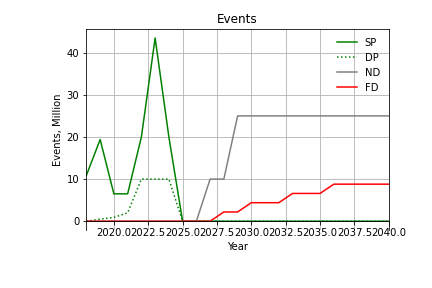
\includegraphics[width=0.8\textwidth]{IntroFigures/Events.png}
\end{dunefigure}

CPU and size/readout are drawn from the above estimates. We then make the following assumptions about data sizes and retention.  
Figures \ref{fig:est:disk,fig:est:tape,fig:est:cores} illustrate the estimated storage and CPU needs through 2030.  In the early years, \dword{pd} and \dword{nd} prototype tests dominate while commissioning and operation of the first (and second) \dword{fd} and the \dword{nd} become important after 2026. 

\begin{itemize}
\item Two copies of raw data are retained indefinitely
\item Commissioning data is marked test and one copy is retained on disk for 6 months. 
\item Reconstruction is performed on the full data sample once/year and 2 copies are retained on disk for 2 years.  
\item Analysis includes calibration and is  equivalent to reconstruction but produces smaller outputs. 
\end{itemize}

\begin{dunefigure}
[Disk estimates]
{fig:est:disk}
{Estimated size of various samples in PB. This estimate includes retention policies and multiple copies.}
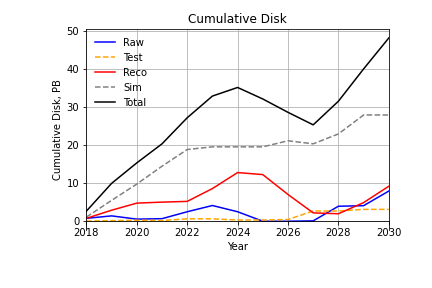
\includegraphics[width=0.8\textwidth]{IntroFigures/Cumulative-Disk.png}
\end{dunefigure}

\begin{dunefigure}
[Tape estimates]
{fig:est:tape}
{Estimated size of various samples in PB. This estimate includes retention policies and multiple copies.}
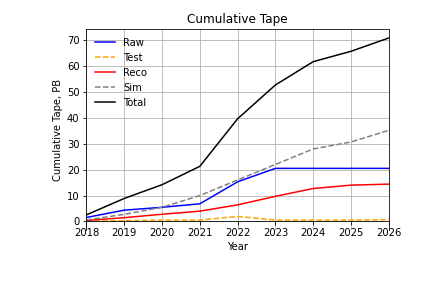
\includegraphics[width=0.8\textwidth]{IntroFigures/Cumulative-Tape.png}
\end{dunefigure}

\begin{dunefigure}
[Tape estimates]
{fig:est:cores}
{Estimated CPU needs for  various samples.  The units are present day cores assuming 70\% efficiency.}
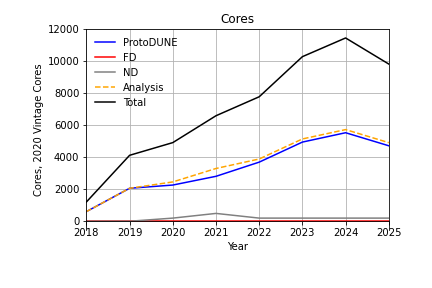
\includegraphics[width=0.8\textwidth]{IntroFigures/Cores.png}
\end{dunefigure}
\end{document}